\section{Model - Exogenous Fertility}

\begin{equation}
    \textbf{State space: }\statespace = \R^{2} \times \{0, 1, 2, 3, 4, 5\} \times \{ 18, 19, \cdots, 70\}
\end{equation}

\begin{equation}
    \textbf{Action space: }\actionspace  = 46 \cdot \{0, 15, 25, 37, 45\} 
\end{equation}

\begin{equation}
    \textbf{States: }\{G, Z, K, Q\}, \qquad \textbf{Actions: } \{H\} 
\end{equation}

The model represents the labour supply of married women - and the effect of children. More precisely it models a woman who can accumulate human capital by supplying a desired number of working hours. The woman can with a certain probability in each period give birth to a child, where, the number of children influences the utility. The model presented here has 4 states: $G$ which represents human capital, $Z$ which represents the agents idiosyncratic wage path, $K$ the number of kids owned by the agent and $Q$ which evolves in a deterministic fashion and represents the age of the agent. The action the agent can take in each period is a discrete number of working hours $H$.

\begin{equation}
    \textbf{Variables: }\{S, W, Y, M, U, L\},  \qquad \textbf{Parameters: } \{\beta_K, \beta_L, \beta_Y, p_\psi, \sigma_\epsilon, \delta, \zeta\}
\end{equation}


To elaborate the rest of the model variables: $U$ is the utility. Following the formulation of (Adda, Dustman, Stevens - The Career Cost of Children XXX), dividing the utility into sub-utility functions, where each sub-utility function allows for curvature by specifying a constant relative risk-averse (CRRA) function for each sub-utility. Assuming the special case of $\ln(\cdot)$. The parameters $\beta_K, \beta_L, \beta_YK$ is the individual weighing of the different sub-utilities. Note that for identification I will restrict $\beta_Y= 1$. $W_t$ the wage for given year as function of the supplied working hours and hourly salary $S$. The hourly Salary has three components: the minimum wage: $\zeta=120$, $G_t$ the human capital and at last $Z_t$ the idiosyncratic wage path. I assume that the three parts are additive. $Y_t$ represents the households total earning, where $M_t$ is the earnings of the husband, $W_t$ mentioned above is the salary of the woman. Lastly $M_t$, the husbands wage is assumed to be a deterministic function of age. It is modelled non parametric using data from Danmarks Statistik Bank.

The states of the agent evolves the following way: $Q_t$ evolves deterministcally. $K_t$ evolves by with a certain probability and ekstra children is added to the household. This probability is dependent on the age of the women $Q$. The idiosyncratic wage path of the women follows a random walk. The Human capital accumulates with a constant depreciation rate $\delta$. adding the number of working hours last period.

\begin{align}
    U_t(K_t, L_t, Y_t) &= \beta_K \ln(K_t) + \beta_L \ln(L_t) + \beta_Y \ln(Y_t) \\
    W_t(S_t, H_t) &=S_t \cdot H_t \\
    S_t(Z_t, G_t) &= \min(\zeta, (\zeta + Z_t + G_t))  \\
    Y_t(W_t, M_t) &= W_t + M_t\\
    M_t(Q_t) &= f^M(Q_t) \\
\end{align}


Law of Motion.

\begin{align}
    Q_{t+1}(Q_t) &= Q_t \\
    K_{t+1}(K_t, Q_t)  &= K_{t} + \psi_t, \qquad \psi_t \sim Bernoulli(p_\psi) \mid Q_t \\
    Z_{t+1}(Z_t) &= Z_t + \epsilon_t, \qquad \epsilon_t \sim \ndist(0, \sigma_\epsilon) \\
    G_{t+1}(G_t) &= G_t(1 - \delta) + H_t \\
\end{align}


\begin{figure}
    \centering
    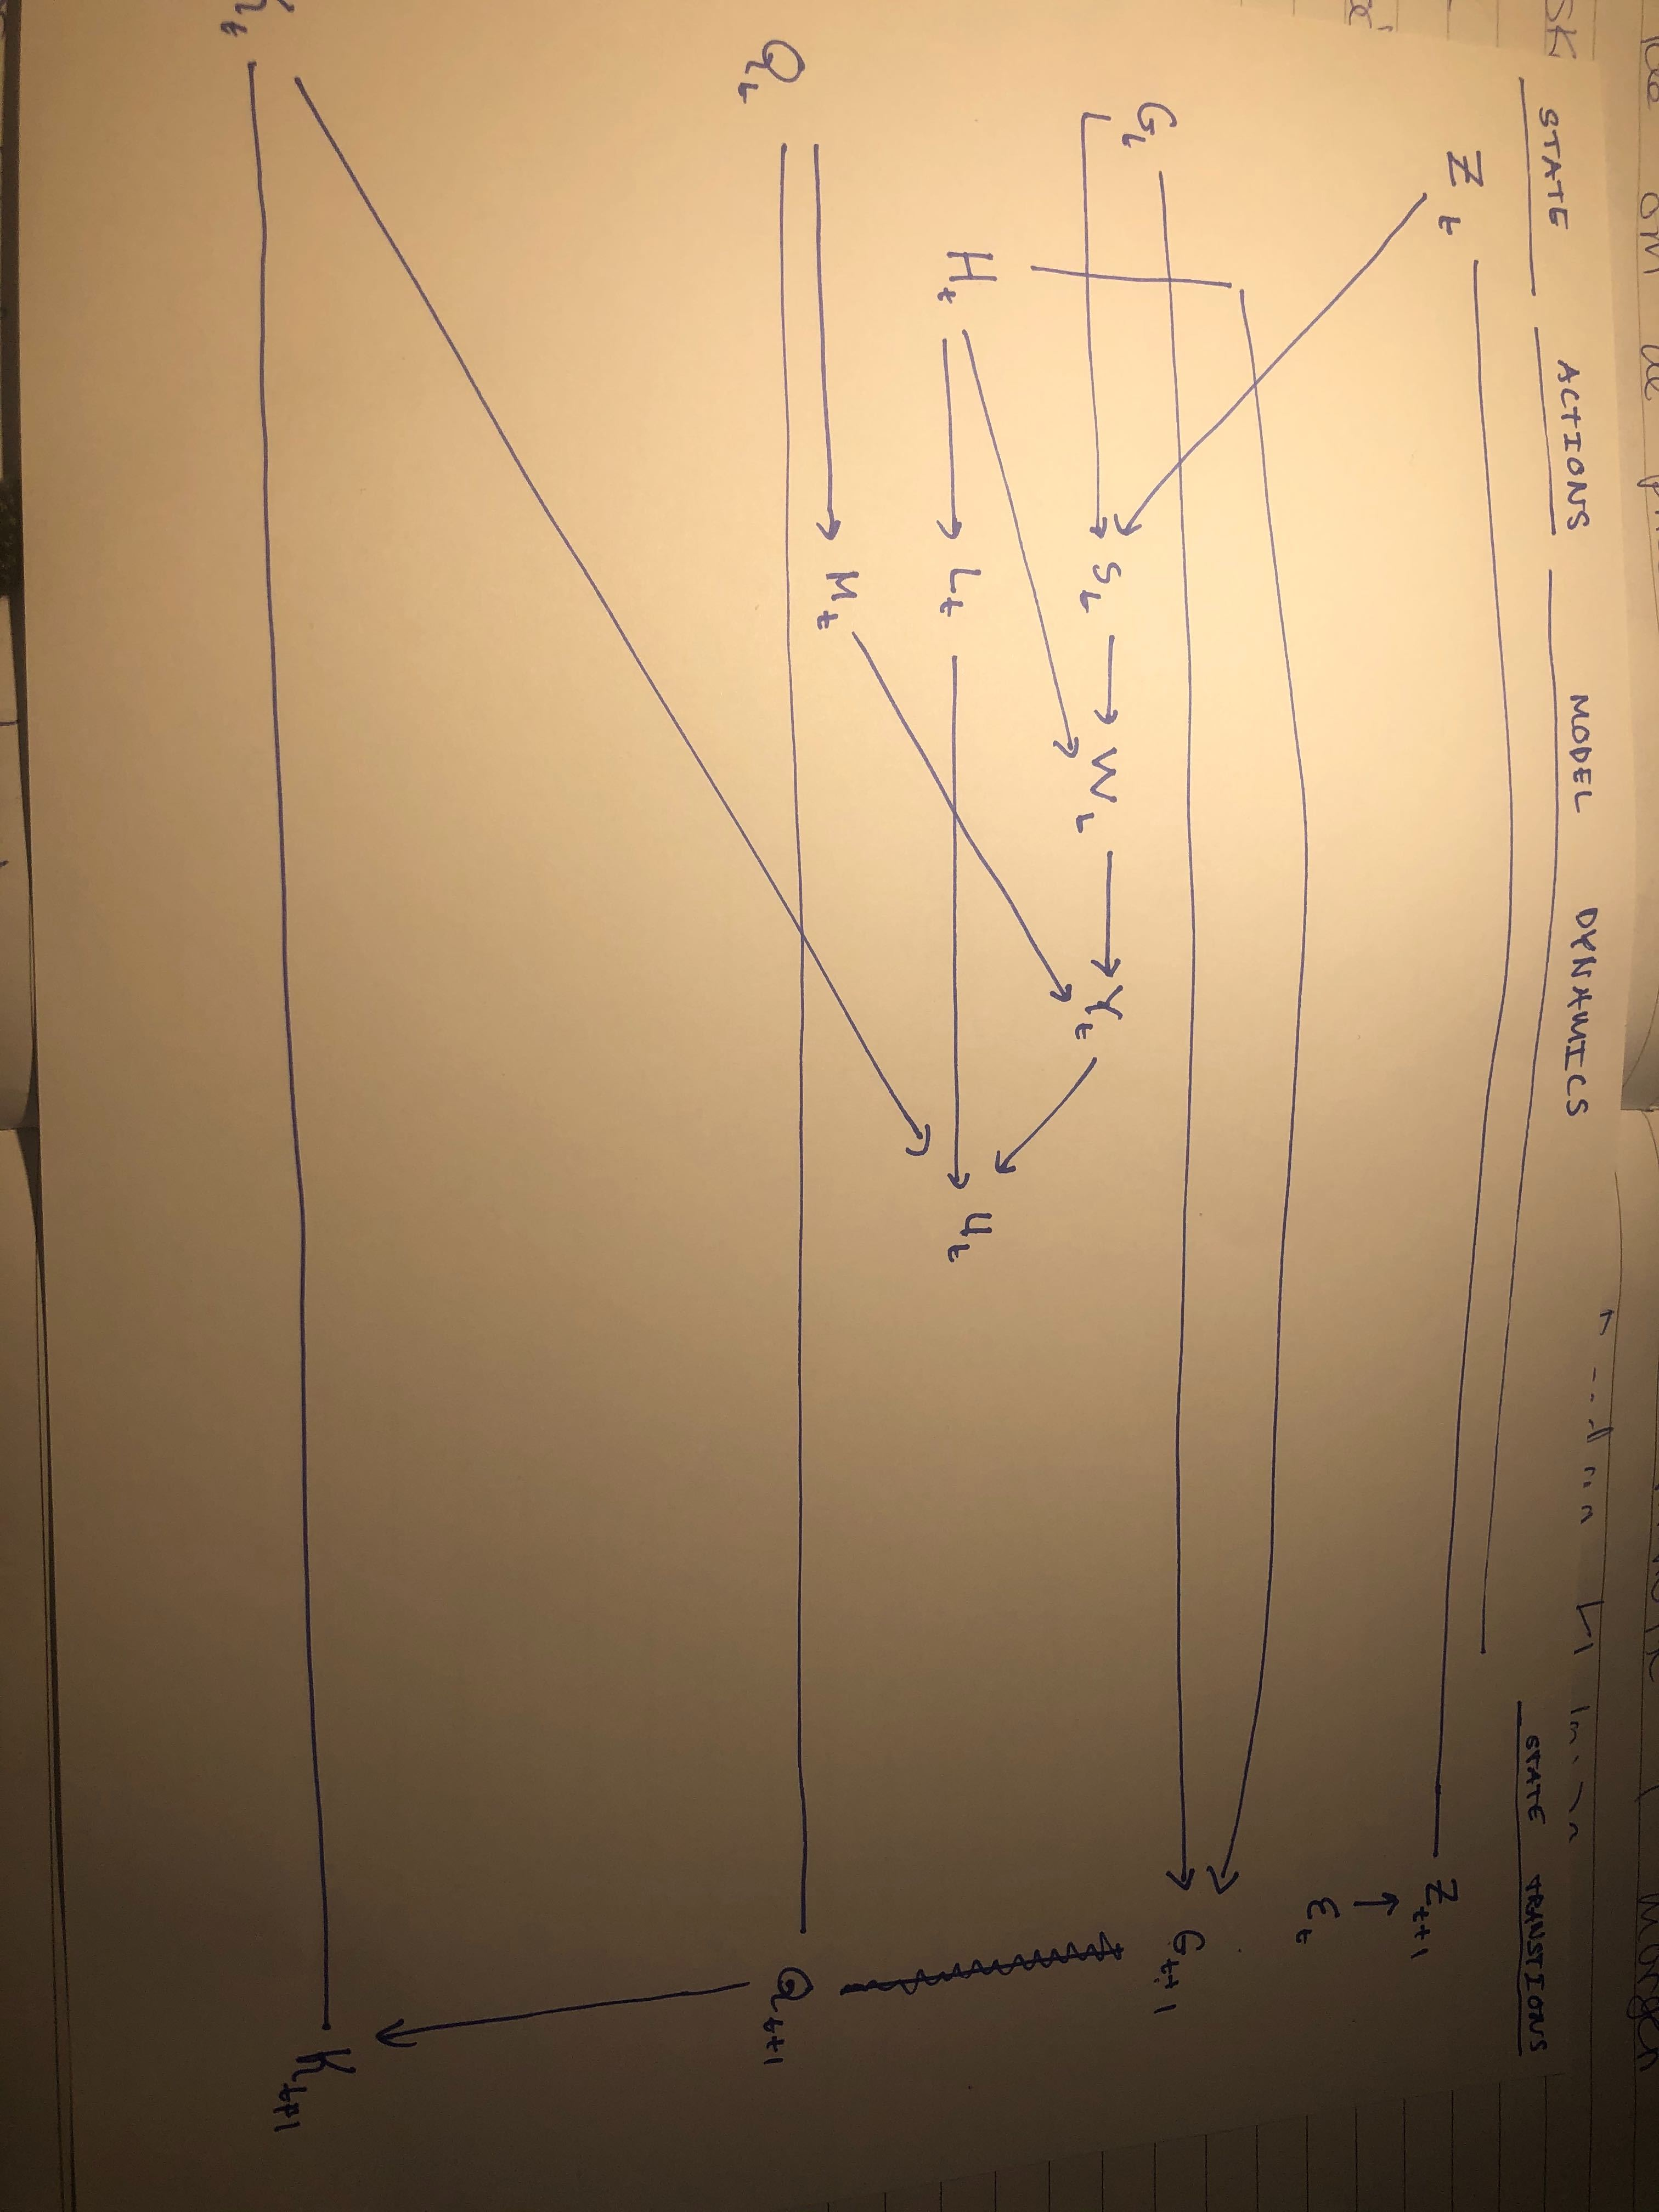
\includegraphics[scale=0.1, angle=90]{figures/modeldynamic_tmp_exogenous.jpg}
    \caption{Model dynamics - Exogenous (TMP)}
    \label{fig:tmp_modeldynamics_exogenous}
\end{figure}